\documentclass[aspectratio=169]{beamer}

% Minimal theme
\usetheme{default}
\usecolortheme{default}
\setbeamertemplate{navigation symbols}{}
\setbeamertemplate{footline}[frame number]

% Dark color scheme - black background with red accents
\definecolor{darkbg}{HTML}{000000}
\definecolor{lighttext}{HTML}{999999}
\definecolor{miamired}{HTML}{941728}
\definecolor{codebg}{HTML}{1a1a1a}

\setbeamercolor{background canvas}{bg=darkbg}
\setbeamercolor{normal text}{fg=lighttext}
\setbeamercolor{frametitle}{fg=miamired}
\setbeamercolor{title}{fg=miamired}
\setbeamercolor{structure}{fg=miamired}
\setbeamercolor{item}{fg=miamired}
\setbeamercolor{block title}{fg=miamired,bg=codebg}
\setbeamercolor{block body}{fg=lighttext,bg=codebg}

% Bold fonts for titles
\setbeamerfont{title}{series=\bfseries,size=\Large}
\setbeamerfont{frametitle}{series=\bfseries}

% Packages
\usepackage{graphicx}
\usepackage{listings}
\usepackage{tikz}
\usepackage{array}
\usepackage{booktabs}
\usepackage{colortbl}

% Code listings style
\lstset{
    basicstyle=\ttfamily\small\color{lighttext},
    backgroundcolor=\color{codebg},
    keywordstyle=\color[HTML]{569cd6},
    commentstyle=\color[HTML]{6a9955},
    stringstyle=\color[HTML]{ce9178},
    showstringspaces=false,
    breaklines=true,
    frame=single,
    rulecolor=\color{codebg}
}

% Table style
\setlength{\arrayrulewidth}{0.5pt}
\arrayrulecolor{miamired}

% Make bold text white
\renewcommand{\textbf}[1]{\textcolor{white}{\bfseries #1}}

% Title
\title{N-Gram Language Models}
\subtitle{Generating Text Without Neural Networks!}
\author{CSE 534}
\date{}

\begin{document}

% Title slide
\begin{frame}
\titlepage
\begin{center}
\textbf{Goal:} Build a simple text generator using just probability and counting

\textbf{No training GPUs needed} - just count character frequencies
\end{center}
\end{frame}

% What is an N-Gram?
\begin{frame}[c]{What is an N-Gram?}
\textbf{N-gram:} Sequence of N consecutive items (characters, words, tokens)

\vspace{1em}
\textbf{Examples with ``hello␣world'':}
\begin{itemize}
    \item \textbf{1-gram (unigram):} \texttt{h}, \texttt{e}, \texttt{l}, \texttt{l}, \texttt{o}, \texttt{␣}, \texttt{w}, \texttt{o}, \texttt{r}, \texttt{l}, \texttt{d}
    \item \textbf{2-gram (bigram):} \texttt{he}, \texttt{el}, \texttt{ll}, \texttt{lo}, \texttt{o␣}, \texttt{␣w}, \texttt{wo}, \texttt{or}, \texttt{rl}, \texttt{ld}
    \item \textbf{3-gram (trigram):} \texttt{hel}, \texttt{ell}, \texttt{llo}, \texttt{lo␣}, \texttt{o␣w}, \texttt{␣wo}, \texttt{wor}, \texttt{orl}, \texttt{rld}
\end{itemize}
\end{frame}

% N-Grams for Text Generation
\begin{frame}[c,fragile]{N-Grams for Text Generation}
\textbf{Idea:} Use previous N-1 characters to predict next character

\vspace{1em}
\begin{columns}[T]
\begin{column}{0.48\textwidth}
\textbf{N-grams from a large corpus (including ``hello''):}

\vspace{0.5em}
\begin{tabular}{|l|r|}
\hline
\rowcolor{codebg}
n-gram & count \\
\hline
\textasciicircum\textasciicircum h & 30 \\
\textasciicircum he & 10 \\
hel & 5 \\
... & ... \\
\hline
\end{tabular}
\end{column}

\begin{column}{0.48\textwidth}
\textbf{Current state:}
\begin{lstlisting}[language=]
Generated: ^^
\end{lstlisting}
\end{column}
\end{columns}
\end{frame}

% Generation Step 1
\begin{frame}[c,fragile]{Generation Step 1}
\begin{columns}[c]
\begin{column}{0.48\textwidth}
\textbf{Trigrams starting with ``\textasciicircum\textasciicircum'':}

\vspace{0.5em}
\begin{tabular}{|l|r|}
\hline
\rowcolor{codebg}
n-gram & count \\
\hline
\textasciicircum\textasciicircum h & 30 \\
\textasciicircum\textasciicircum w & 10 \\
\textasciicircum\textasciicircum j & 10 \\
... & ... \\
\hline
\end{tabular}

\vspace{0.5em}
\textbf{Total: 50}
\end{column}

\begin{column}{0.48\textwidth}
\textbf{Generated so far:} \texttt{\textasciicircum\textasciicircum}\\
\textbf{Current context:} \texttt{\textasciicircum\textasciicircum}

\vspace{0.5em}
\textbf{Probabilities:}

\begin{tabular}{@{}l@{ }l@{ }l@{}}
h & \textcolor{miamired}{\rule{3.6cm}{0.3cm}} & 30/50 \\
w & \textcolor{miamired}{\rule{1.2cm}{0.3cm}} & 10/50 \\
j & \textcolor{miamired}{\rule{1.2cm}{0.3cm}} & 10/50
\end{tabular}

\vspace{0.5em}
\textbf{Selected: h}
\end{column}
\end{columns}
\end{frame}

% Generation Step 2
\begin{frame}[c,fragile]{Generation Step 2}
\begin{columns}[c]
\begin{column}{0.48\textwidth}
\textbf{Trigrams starting with ``\textasciicircum h'':}

\vspace{0.5em}
\begin{tabular}{|l|r|}
\hline
\rowcolor{codebg}
n-gram & count \\
\hline
\textasciicircum he & 10 \\
\textasciicircum ho & 8 \\
\textasciicircum ha & 5 \\
\textasciicircum hi & 5 \\
... & ... \\
\hline
\end{tabular}

\vspace{0.5em}
\textbf{Total: 28}
\end{column}

\begin{column}{0.48\textwidth}
\textbf{Generated so far:} \texttt{\textasciicircum\textasciicircum h}\\
\textbf{Current context:} \texttt{\textasciicircum h}

\vspace{0.5em}
\textbf{Probabilities:}

\begin{tabular}{@{}l@{ }l@{ }l@{}}
e & \textcolor{miamired}{\rule{3.0cm}{0.3cm}} & 10/28 \\
o & \textcolor{miamired}{\rule{2.4cm}{0.3cm}} & 8/28 \\
a & \textcolor{miamired}{\rule{1.5cm}{0.3cm}} & 5/28 \\
i & \textcolor{miamired}{\rule{1.5cm}{0.3cm}} & 5/28
\end{tabular}

\vspace{0.5em}
\textbf{Selected: e}
\end{column}
\end{columns}
\end{frame}

% Generation Step 3
\begin{frame}[c,fragile]{Generation Step 3}
\begin{columns}[c]
\begin{column}{0.48\textwidth}
\textbf{Trigrams starting with ``he'':}

\vspace{0.5em}
\begin{tabular}{|l|r|}
\hline
\rowcolor{codebg}
n-gram & count \\
\hline
hel & 5 \\
her & 3 \\
hey & 2 \\
... & ... \\
\hline
\end{tabular}

\vspace{0.5em}
\textbf{Total: 10}
\end{column}

\begin{column}{0.48\textwidth}
\textbf{Generated so far:} \texttt{\textasciicircum\textasciicircum he}\\
\textbf{Current context:} \texttt{he}

\vspace{0.5em}
\textbf{Probabilities:}

\begin{tabular}{@{}l@{ }l@{ }l@{}}
l & \textcolor{miamired}{\rule{3.0cm}{0.3cm}} & 5/10 \\
r & \textcolor{miamired}{\rule{1.8cm}{0.3cm}} & 3/10 \\
y & \textcolor{miamired}{\rule{1.2cm}{0.3cm}} & 2/10
\end{tabular}

\vspace{0.5em}
\textbf{Selected: l}
\end{column}
\end{columns}
\end{frame}

% Generation Step 4
\begin{frame}[c,fragile]{Generation Step 4}
\begin{columns}[c]
\begin{column}{0.48\textwidth}
\textbf{Trigrams starting with ``el'':}

\vspace{0.5em}
\begin{tabular}{|l|r|}
\hline
\rowcolor{codebg}
n-gram & count \\
\hline
ell & 25 \\
els & 8 \\
ele & 5 \\
... & ... \\
\hline
\end{tabular}

\vspace{0.5em}
\textbf{Total: 38}
\end{column}

\begin{column}{0.48\textwidth}
\textbf{Generated so far:} \texttt{\textasciicircum\textasciicircum hel}\\
\textbf{Current context:} \texttt{el}

\vspace{0.5em}
\textbf{Probabilities:}

\begin{tabular}{@{}l@{ }l@{ }l@{}}
l & \textcolor{miamired}{\rule{4.0cm}{0.3cm}} & 25/38 \\
s & \textcolor{miamired}{\rule{1.6cm}{0.3cm}} & 8/38 \\
e & \textcolor{miamired}{\rule{1.0cm}{0.3cm}} & 5/38
\end{tabular}

\vspace{0.5em}
\textbf{Selected: l}
\end{column}
\end{columns}
\end{frame}

% Generation Step 5
\begin{frame}[c,fragile]{Generation Step 5}
\begin{columns}[c]
\begin{column}{0.48\textwidth}
\textbf{Trigrams starting with ``ll'':}

\vspace{0.5em}
\begin{tabular}{|l|r|}
\hline
\rowcolor{codebg}
n-gram & count \\
\hline
llo & 15 \\
lly & 12 \\
lle & 8 \\
... & ... \\
\hline
\end{tabular}

\vspace{0.5em}
\textbf{Total: 35}
\end{column}

\begin{column}{0.48\textwidth}
\textbf{Generated so far:} \texttt{\textasciicircum\textasciicircum hell}\\
\textbf{Current context:} \texttt{ll}

\vspace{0.5em}
\textbf{Probabilities:}

\begin{tabular}{@{}l@{ }l@{ }l@{}}
o & \textcolor{miamired}{\rule{3.4cm}{0.3cm}} & 15/35 \\
y & \textcolor{miamired}{\rule{2.7cm}{0.3cm}} & 12/35 \\
e & \textcolor{miamired}{\rule{1.8cm}{0.3cm}} & 8/35
\end{tabular}

\vspace{0.5em}
\textbf{Selected: o}

\vspace{0.5em}
\textbf{Final result:} \texttt{\textasciicircum\textasciicircum hello}
\end{column}
\end{columns}
\end{frame}

% Why Does This Work?
\begin{frame}{Why Does This Work?}
\textbf{We just generated text by counting!} But why does this actually work?

\vspace{1em}
\textbf{The Theory:}

\begin{itemize}
    \item<1-> \textbf{Autoregressive view:} Generation proceeds one step at a time, conditioning on prior context
    \item<2-> Many generative models rely on $P(\text{next} \mid \text{context})$ or an equivalent conditional target
    \item<3-> N-grams are a simple, interpretable example of the same probability ideas used in language modeling
    \item<4-> This helps build intuition for more complex models, even though diffusion, grammars, and transformers use different mechanisms
\end{itemize}
\end{frame}

% Probability: Joint vs Conditional
\begin{frame}[c]{Probability: Joint vs Conditional}
Let's put this into the context of generative modeling.\\
We are learning a model for $p(\text{sequence})$.

\vspace{1em}
\textbf{Goal:} Model probability of entire sequence

\vspace{0.5em}
\textbf{Example:} $p(\text{hello}) = p(h, e, l, l, o)$
\end{frame}

% Chain Rule - Step by Step
\begin{frame}{Chain Rule - Step by Step}
\textbf{Chain rule} factorizes joint into conditionals:

\vspace{1em}
\onslide<1->{
$$p(\text{hello}) = \underbrace{p(h)}_{\text{easy!}} \cdot p(\text{ello}|h)$$
}

\vspace{0.5em}
\onslide<2->{
$$p(\text{hello}) = p(h) \cdot p(e|h) \cdot p(\text{llo}|\text{he})$$
}

\vspace{0.5em}
\onslide<3->{
$$p(\text{hello}) = p(h) \cdot p(e|h) \cdot p(l|\text{he}) \cdot p(\text{lo}|\text{hel})$$
}

\vspace{0.5em}
\onslide<4->{
$$p(\text{hello}) = p(h) \cdot p(e|h) \cdot p(l|\text{he}) \cdot p(l|\text{hel}) \cdot p(o|\text{hell})$$
}
\end{frame}

% Chain Rule Visualization
\begin{frame}{Chain Rule Visualization}
\centering
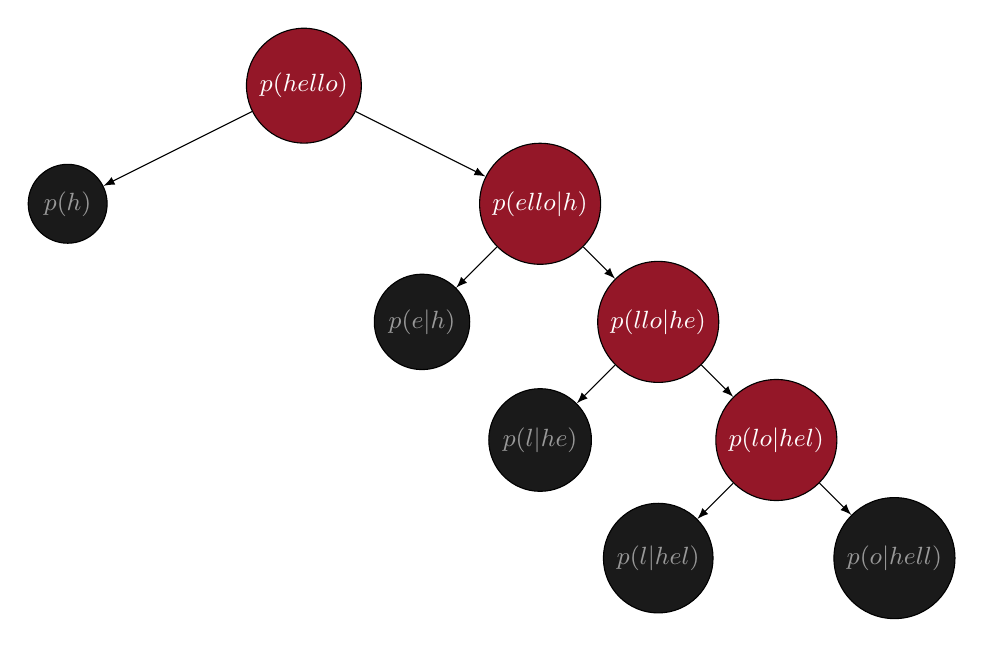
\begin{tikzpicture}[
    level 1/.style={sibling distance=6cm,level distance=1.5cm},
    level 2/.style={sibling distance=3cm,level distance=1.5cm},
    level 3/.style={sibling distance=3cm,level distance=1.5cm},
    every node/.style={circle,draw,minimum size=0.8cm,font=\small},
    edge from parent/.style={draw,-latex}
]
\node[fill=miamired,text=white] {$p(\text{hello})$}
    child {node[fill=codebg,text=lighttext] {$p(h)$}}
    child {node[fill=miamired,text=white] {$p(\text{ello}|h)$}
        child {node[fill=codebg,text=lighttext] {$p(e|h)$}}
        child {node[fill=miamired,text=white] {$p(\text{llo}|\text{he})$}
            child {node[fill=codebg,text=lighttext] {$p(l|\text{he})$}}
            child {node[fill=miamired,text=white] {$p(\text{lo}|\text{hel})$}
                child {node[fill=codebg,text=lighttext] {$p(l|\text{hel})$}}
                child {node[fill=codebg,text=lighttext] {$p(o|\text{hell})$}}
            }
        }
    };
\end{tikzpicture}
\end{frame}

% General Pattern
\begin{frame}{General Pattern}
$$p(x_1,\ldots,x_n) = p(x_1) \cdot p(x_2|x_1) \cdot p(x_3|x_1,x_2) \cdots p(x_n|x_1,\ldots,x_{n-1})$$

\vspace{1em}
\textbf{Problem:} $p(x_n|x_1,\ldots,x_{n-1})$ needs \textbf{entire history}

\begin{itemize}
    \item<1-> For long sequences: too many possible histories!
    \item<2-> As context gets longer, harder to find enough matches in training data
\end{itemize}
\end{frame}

% Markov Assumption
\begin{frame}{Markov Assumption}
\textbf{Key idea:} Assume each character depends only on \textbf{last k characters}

\vspace{1em}
$$p(x_n|x_1,\ldots,x_{n-1}) \approx p(x_n|x_{n-k},\ldots,x_{n-1})$$
\end{frame}

% Markov Assumption (continued)
\begin{frame}{Markov Assumption (continued)}
\textbf{Order-k Markov assumption:}

\begin{itemize}
    \item<1-> Ignore history beyond k positions
    \item<2-> Only use k previous characters as context
\end{itemize}

\vspace{1em}
\onslide<3->{
\textbf{Example with k=2:}
$$p(\text{hello}) = p(h) \cdot p(e|h) \cdot p(l|\text{he}) \cdot \underbrace{p(l|\text{el})}_{\text{no 'h'!}} \cdot \underbrace{p(o|\text{ll})}_{\text{no 'he'!}}$$
}
\end{frame}

% All Models Are Wrong
\begin{frame}{``All Models Are Wrong, But Some Are Useful''}
\begin{columns}[c]
\begin{column}{0.55\textwidth}
\textbf{George Box (Statistician)}

\vspace{1em}
Every model makes simplifying assumptions

\vspace{0.5em}
\textbf{Our Markov assumption:}
\begin{itemize}
    \item<1-> Only last $k$ characters matter
    \item<2-> Ignore all earlier context
    \item<3-> This is \textbf{wrong}... but \textbf{useful}!
\end{itemize}
\end{column}

\begin{column}{0.40\textwidth}
\centering
\fcolorbox{miamired}{codebg}{
\begin{minipage}{0.9\textwidth}
\centering
\vspace{0.5em}
\textit{``All models are wrong,\\
but some are useful''}

\vspace{0.5em}
--- George Box
\vspace{0.5em}
\end{minipage}
}
\end{column}
\end{columns}
\end{frame}

% Inductive Bias and Limitations
\begin{frame}[fragile]{Inductive Bias and Limitations}
\textbf{Fixed context window = structural constraint (inductive bias)}

\vspace{0.5em}
\textbf{The model cannot learn:}

\begin{itemize}
    \item<1-> \textbf{Long-range dependencies:} Matching quotes 100 chars apart
    \item<2-> \textbf{Palindromes:} No understanding of symmetry
    \item<3-> \textbf{Hierarchical structure:} Nested parentheses or balanced brackets
    \item<4-> \textbf{Pattern repetition:} Train on ``bonbon'' $\to$ ``bonbonbonbon...'' forever!
    \item<5-> \textbf{Sparse contexts:} \texttt{``To be or''} appears rarely in Shakespeare
    \item<6-> \textbf{Dead ends:} Typo or rare prefix $\to$ no continuation $\to$ \texttt{STOP}
\end{itemize}

\vspace{0.5em}
\onslide<7->{
\textbf{Trade-off:} Larger $k$ needs exponentially more data (vocab$^k$ contexts)

\vspace{0.3em}
\small Modern transformers use learned attention to relax these constraints
}
\end{frame}

% Bayesian Smoothing
\begin{frame}{Bayesian Smoothing: Handling Unseen Contexts}
\textbf{Problem:} What if we encounter a context we never saw in training?

\vspace{1em}
\textbf{Without smoothing:} $p(x|c) = 0$ for unseen pairs $\to$ \texttt{STOP} or infinite loss

\vspace{1em}
\onslide<2->{
\textbf{Bayesian idea:} Combine prior belief with observed data

\vspace{0.5em}
$$p(\mu | D) = \frac{p(D | \mu) \cdot p(\mu)}{p(D)}$$

\vspace{0.5em}
\begin{itemize}
    \item<3-> $p(\mu)$ = \textbf{prior}: belief before seeing data
    \item<4-> $p(D|\mu)$ = \textbf{likelihood}: how well data fits model
    \item<5-> $p(\mu|D)$ = \textbf{posterior}: updated belief after seeing data
\end{itemize}

\vspace{0.5em}
\onslide<6->{
\small (Full conjugate prior theory is for advanced courses)
}
}
\end{frame}

% Prior as Imaginary Experiments
\begin{frame}{Prior as Imaginary Experiments}
\textbf{Intuition:} Pretend we did $\alpha$ "prior experiments" with uniform results

\vspace{1em}
\textbf{Smoothing formula:}
$$\hat{p}(x|c) = \frac{\text{count}(c,x) + \alpha}{\text{count}(c) + \alpha \cdot |\text{vocab}|}$$

\vspace{1em}
\onslide<2->{
\textbf{Interpretation:}
\begin{itemize}
    \item<2-> Imagine we did $\alpha$ experiments before training
    \item<3-> Each experiment produced a uniform distribution over all characters
    \item<4-> $\alpha$ doesn't have to be an integer! We can use $\alpha = 0.01$
    \item<5-> This adds $\alpha$ "virtual counts" for each character
\end{itemize}
}
\end{frame}

% Choosing Alpha
\begin{frame}{Choosing $\alpha$: How Much to Trust the Prior}
\textbf{How much weight should we give to the prior?}

\vspace{1em}
\begin{itemize}
    \item<1-> $\alpha = 1$: Add-one (Laplace) smoothing—1 uniform experiment per character
    \item<2-> $\alpha = 0.01$: Weak prior—0.01 uniform experiments per character
    \item<3-> Smaller $\alpha$ = trust real data more, imaginary prior less
\end{itemize}

\vspace{1em}
\onslide<4->{
\textbf{Example with vocab size 100:}
\begin{itemize}
    \item<5-> $\alpha = 1$: Equivalent to 100 prior observations (too strong!)
    \item<6-> $\alpha = 0.01$: Equivalent to 1 prior observation total
    \item<7-> Prevents division by zero without overwhelming real data
\end{itemize}

\vspace{0.5em}
\onslide<8->{
\textbf{Rule of thumb:} $\alpha \ll 1$ prevents gibberish while trusting your corpus
}
}
\end{frame}

% Training: Count N-Grams
\begin{frame}[fragile]{Training: Count N-Grams}
\textbf{Step 1:} Fetch corpus (Shakespeare plays)

\begin{lstlisting}[language=Python]
from urllib.request import urlopen

url = "https://raw.githubusercontent.com/karpathy/\
char-rnn/master/data/tinyshakespeare/input.txt"
with urlopen(url) as r:
    corpus = r.read().decode('utf-8')
\end{lstlisting}

\vspace{1em}
\textbf{Step 2:} Define parameters

\begin{lstlisting}[language=Python]
ORDER = 8   # context length (8-char context -> 9-gram)
PAD = "^"   # padding at start
END = "$"   # end marker
\end{lstlisting}
\end{frame}

% Training: Counting Loop
\begin{frame}[fragile,shrink=5]{Training: Counting Loop}
\textbf{Step 3:} Count frequencies

\begin{lstlisting}[language=Python]
count = {}  # count[context] = {next_char: frequency}

for block in blocks:
    seq = PAD * ORDER + block + END  # pad start, mark end
    
    for i in range(len(seq) - ORDER):
        ctx = seq[i:i+ORDER]          # 8 characters
        next_char = seq[i+ORDER]       # 1 character
        
        if ctx not in count:
            count[ctx] = {}
        count[ctx][next_char] = \
            count[ctx].get(next_char, 0) + 1
\end{lstlisting}
\end{frame}


% Training: Save Model
\begin{frame}[fragile]{Training: Save Model}
\textbf{Step 4:} Save counts

\begin{lstlisting}[language=Python]
import json

with open("ngram_counts.json", "w") as f:
    json.dump(count, f)
\end{lstlisting}

\vspace{0.5em}
\textbf{Result:} Dictionary mapping contexts to character frequencies
\begin{lstlisting}[language=]
{
  "^^^^^^^^": {"T": 100, "A": 50, ...},
  "^^^^^^^T": {"o": 80, "h": 20, ...},
  ...
  "To be or": {"n": 42, " ": 15, "d": 3},
  "be or no": {"t": 87},
  ...
}
\end{lstlisting}
\vspace{1em}
\textbf{Key insight:} We've estimated $p(\text{next\_char} \mid \text{context})$ by \textbf{counting!}
\end{frame}

% Prediction: Load and Initialize
\begin{frame}[fragile]{Prediction: Load and Initialize}
\textbf{Step 1:} Load counts

\begin{lstlisting}[language=Python]
with open("ngram_counts.json") as f:
    count = json.load(f)
\end{lstlisting}

\vspace{1em}
\textbf{Step 2:} Start with padding

\begin{lstlisting}[language=Python]
import numpy as np

rng = np.random.default_rng()
gen = PAD * ORDER  # "^^^^^^^^"
\end{lstlisting}
\end{frame}

% Prediction: Generation Loop
\begin{frame}[fragile,shrink=10]{Prediction: Generation Loop}
\textbf{Step 3:} Generate one character at a time

\begin{lstlisting}[language=Python]
for _ in range(MAX_LEN):
    ctx = gen[-ORDER:]              # last 8 characters
    ctx_counts = count.get(ctx, {}) # get observed frequencies
    
    if not ctx_counts:              # unseen context
        break
    
    # Convert counts to probabilities and sample
    chars = list(ctx_counts.keys())
    probs = np.array([ctx_counts[c] for c in chars])
    probs = probs / probs.sum()     # normalize
    
    next_char = rng.choice(chars, p=probs)
    gen += next_char
    
    if next_char == END:
        break
\end{lstlisting}
\end{frame}


% Prediction: Output
\begin{frame}[fragile]{Prediction: Output}
\textbf{Step 4:} Clean up output

\begin{lstlisting}[language=Python]
# Strip padding and end marker
output = gen[ORDER:].replace(END, "")
print(output)
\end{lstlisting}

\vspace{1em}
\textbf{Example outputs:}
\begin{lstlisting}[language=]
ROMEO:
O, that I were a glove upon that hand,
That I might touch that cheek!

NURSE:
What say you? can you love the gentleman?
\end{lstlisting}

\vspace{1em}
\textbf{Surprisingly coherent} for such a simple model!
\end{frame}

% Live Demo
\begin{frame}[fragile]{Live Demo}
Open terminal and run:
\begin{lstlisting}[language=bash]
cd mathematical_foundations/07_ngram
python 07_ngram_train.py           # count N-grams
python 07_ngram_predict.py         # basic (may hit dead ends)
python 07_ngram_predict_smoothed.py # with Bayesian smoothing
\end{lstlisting}

\vspace{0.5em}
\textbf{Compare outputs:} The smoothed version never stops early
\end{frame}

% Evaluation: Perplexity
\begin{frame}{Evaluation: Perplexity}
\textbf{Recall from last lecture:} Perplexity measures model quality

\vspace{1em}
$$\text{perplexity} = \exp\left(-\frac{1}{T} \sum_{t=1}^{T} \log p(x_t | c_t)\right)$$

\vspace{0.5em}
{\small Note: Using base $e$ (natural log) for mathematical convenience; last lecture used base 2}

\vspace{0.5em}
\textbf{For N-gram models:}
\begin{itemize}
    \item<1-> $c_t$ = the $N-1$ character context at position $t$
    \item<2-> Lower perplexity = better predictions on held-out text
    \item<3-> Compare different $N$ values or smoothing strategies
\end{itemize}

\vspace{0.5em}
\onslide<4->{
\textbf{Trade-off:} Larger $N$ may overfit; smaller $N$ may underfit
}
\end{frame}

% Extensions and Experiments
\begin{frame}[fragile]{Extensions and Experiments}
\textbf{Try different sources:}
\begin{itemize}
    \item \textbf{Pride and Prejudice:} Classic prose style\\
    \small\texttt{gutenberg.org/cache/epub/1342/pg1342.txt}
    \item \textbf{Alice in Wonderland:} Whimsical narrative\\
    \small\texttt{gutenberg.org/cache/epub/11/pg11.txt}
    \item \textbf{Django source:} Python syntax patterns\\
    \small\texttt{raw.githubusercontent.com/django/django/main/django/views/generic/base.py}
\end{itemize}

\vspace{0.5em}
\textbf{Evaluate with perplexity:}
\begin{itemize}
    \item Split data into train/test sets
    \item Compute NLL on held-out text: $-\frac{1}{T} \sum \log p(x_t|c_t)$
    \item Lower perplexity = better predictions
\end{itemize}

\vspace{0.5em}
\textbf{Modify the URL in} \texttt{07\_ngram\_train.py} \textbf{and retrain!}
\end{frame}

% Characters vs Tokens
\begin{frame}[fragile]{Characters vs Tokens}
\begin{columns}[T]
\begin{column}{0.48\textwidth}
\textbf{Current: Character-level}
\begin{itemize}
    \item Fine-grained
    \item Needs less data
    \item Vocab $\approx$ 100 characters
\end{itemize}
\end{column}

\begin{column}{0.48\textwidth}
\textbf{Alternative: Token-level}
\begin{lstlisting}[language=Python]
import tiktoken
enc = tiktoken.get_encoding(
    "cl100k_base"
)
tokens = enc.encode(text)
# Use tokens as keys
\end{lstlisting}
\begin{itemize}
    \item Vocab $\approx$ 50,000 tokens
    \item Needs more data
    \item Better semantic units
\end{itemize}
\end{column}
\end{columns}
\end{frame}

% Varying ORDER Parameter
\begin{frame}{Varying ORDER Parameter}
\begin{tabular}{|c|l|l|}
\hline
\rowcolor{codebg}
ORDER & Pattern Type & Use Case \\
\hline
2 & Simple, generic & Fast generation, minimal data \\
8 & Medium context & What we happened to use \\
20 & Very specific, Shakespeare-like & Huge corpus needed \\
\hline
\end{tabular}

\vspace{1em}
\textbf{Exponential growth:} $\text{vocab}^{\text{ORDER}}$ possible contexts

\vspace{0.5em}
{\small No single "right" ORDER—depends on corpus size and desired specificity}
\end{frame}

% Questions
\begin{frame}[fragile]{Questions?}
\textbf{Try it yourself:}
\begin{lstlisting}[language=bash]
cd mathematical_foundations/07_ngram
python 07_ngram_train.py
python 07_ngram_predict.py         # may hit dead ends
python 07_ngram_predict_smoothed.py # with Bayesian smoothing
\end{lstlisting}

\vspace{1em}
\textbf{Experiment with:}
\begin{itemize}
    \item Different text sources
    \item Different ORDER values
    \item Character vs token-level models
    \item Compare basic vs smoothed generation
\end{itemize}
\end{frame}

\end{document}
